\section{Auswertung}
\label{sec:Auswertung}
\subsection{Vorbereitende Versuche}
Als Vorbereitende Versuche wird die Schallgeschwindigkeit über die Resonanzfrequenzen bestimmt und es wird ein Vergleich gezogen
zwischen der Datennahme mittels Osziloskop und mittels dem Programm \texttt{SpectrumSLC}.
\subsubsection{Bestimmung der Schallgeschwindigkeit}
Aus \eqref{??}[$\lambda$ abhängig von d] kann die Schallgeschwindigkeit über die Differenz der Resonanzfrequenzen
bestimmt werden. Hierfür werden diese gegen die Länge der Röhren aufgetragen. Die Länge der Röhren ist bekannt, da immer Röhren 
der gleichen Länge hinzugefühgt werden.
\FloatBarrier
\begin{table}
    \centering
    \caption{Messwerte für die Bestimmung der Schallgeschwindigkeit}
    \label{tab:Schallgeschwindigkeit}
    \begin{tabular}{c c c c}
        \toprule
        Länge /\SI{}{\milli\meter}& erste Resonanz /\SI{}{\kilo\hertz} & zweite Resonanz /\SI{}{\kilo\hertz}& Differenz /\SI{}{\kilo\hertz}\\
        \midrule
        $\num{50}$&$\num{6.87}$&$\num{10.28}$&$\num{3.41}$\\
        $\num{100}$&$\num{6.89}$&$\num{8.6}$&$\num{1.71}$\\
        $\num{150}$&$\num{6.895}$&$\num{8.05}$&$\num{1.16}$\\
        $\num{200}$&$\num{6.897}$&$\num{7.759}$&$\num{0.86}$\\
        $\num{250}$&$\num{6.9}$&$\num{7.59}$&$\num{0.69}$\\
        $\num{300}$&$\num{6.9}$&$\num{7.477}$&$\num{0.58}$\\
        \bottomrule
    \end{tabular}
\end{table}
\FloatBarrier
Durch die Messwerte aus \ref{tab:Schallgeschwindigkeit} wird die Funktion
\begin{equation*}
    f(x) = a \frac{1}{x} + b
\end{equation*}
gefittet.\\
Mit der Gleichung 
\begin{equation*}
    nc = 2df +b =2a+b
\end{equation*}
kann die Schallgeschwindigkeit bestimmt werden.
\FloatBarrier
\begin{figure}
    \caption{Messwerte und Fitfunktion für die Bestimmung der Schallgeschwindigkeit}
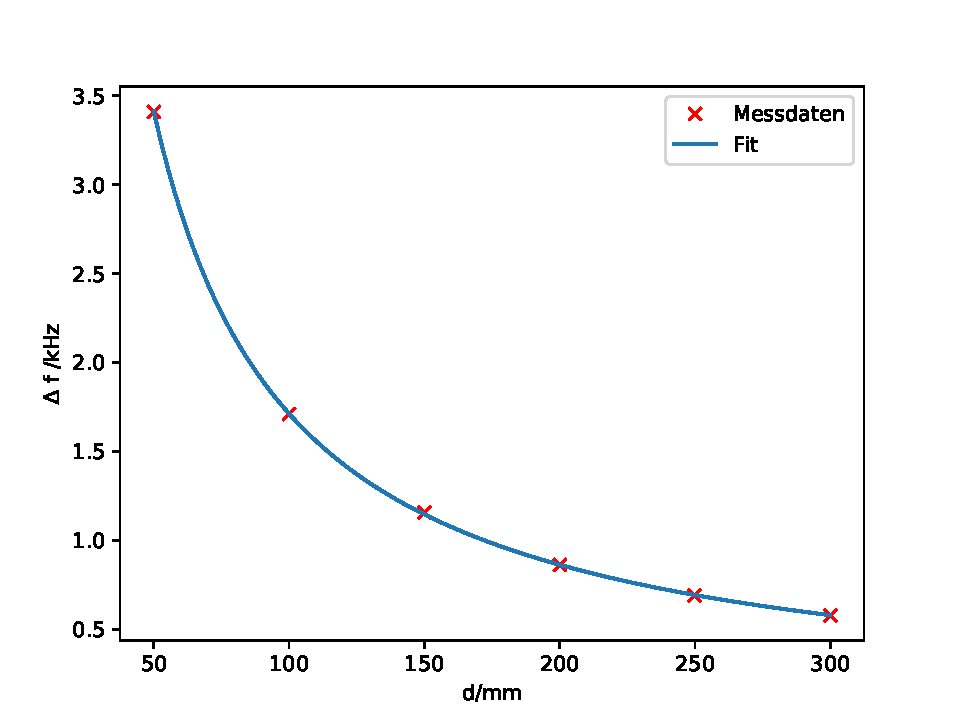
\includegraphics[width = \textwidth]{figure/Schallgeschwindigkeit.pdf}
\end{figure}
\FloatBarrier
Die Parameter der Funktion sind:
\begin{align*}
    a&= \num{169.9(3)}\\
    b&= \num{0.013(3)}
\end{align*}
Daraus kann der Wert $c=\SI{339.8(7)}{\meter\per\second}$ bestimmt werden.

\subsubsection{Vergleich der Datennahme}
Um die beiden Methoden der Datennahme zu testen wird das Spektrum des Zylinders vermessen.
Hierbei wird die Anzahl der Zylinder schrittweise von eins auf sechs erhöht.
\FloatBarrier
\begin{figure}
    \begin{minipage}[b]{.4\linewidth} % [b] => Ausrichtung an \caption
        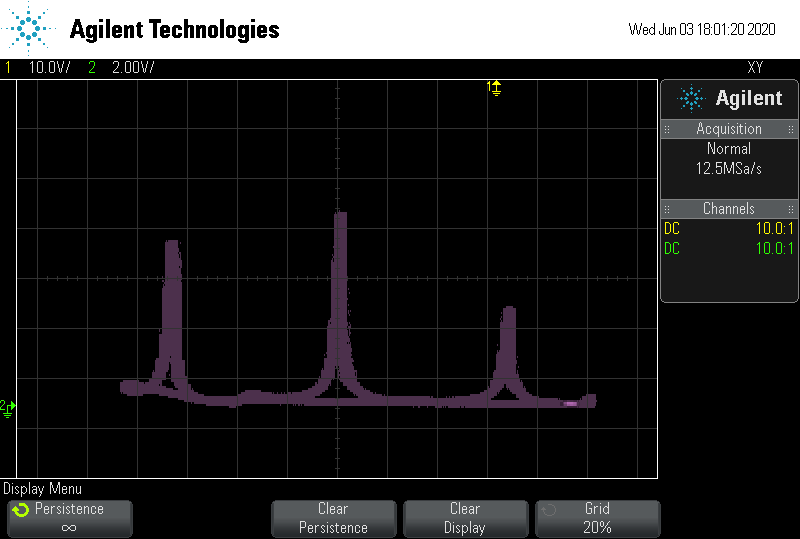
\includegraphics[width=\linewidth]{figure/1Zylinder.png}
        \vspace*{0.008cm}
        \caption{Spektrum von einem Zylinder\\ mittels Osziloskop}
     \end{minipage}
     \hspace{.1\linewidth}% Abstand zwischen Bilder
     \begin{minipage}[b]{.4\linewidth} % [b] => Ausrichtung an \caption
        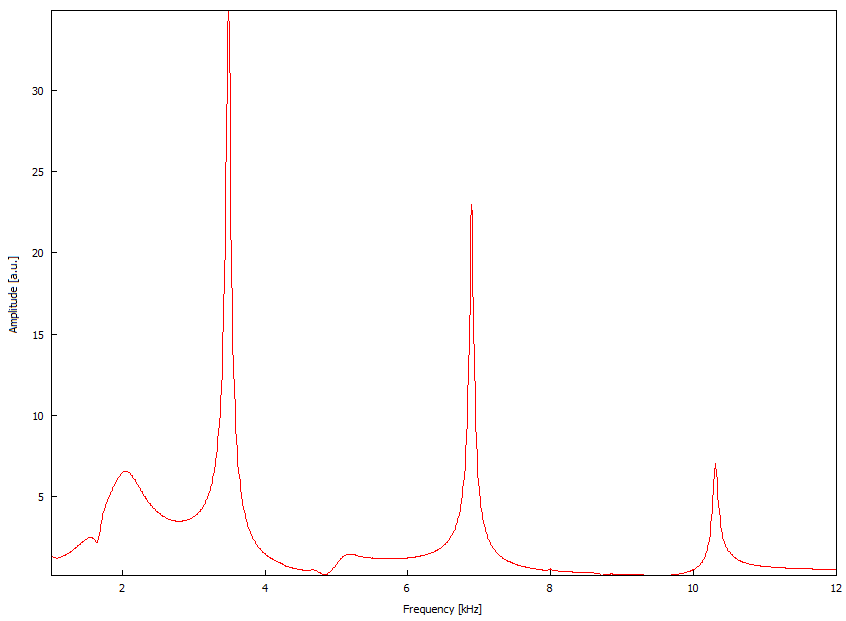
\includegraphics[width=\linewidth]{figure/1_Zylinder.png}
        \caption{Spektrum von einem Zylinder\\ mittels \texttt{SpectrumSLC}}
     \end{minipage}
\end{figure}
%\FloatBarrier
%\FloatBarrier
\begin{figure}
    \begin{minipage}[b]{.4\linewidth} % [b] => Ausrichtung an \caption
        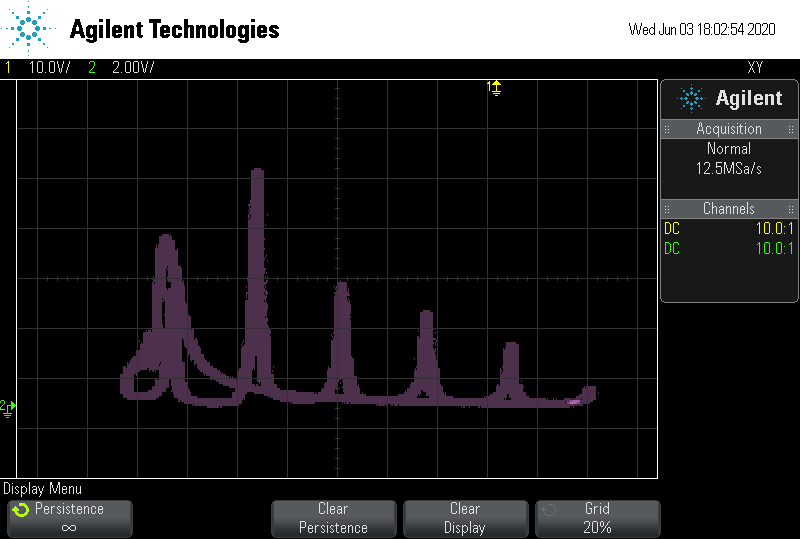
\includegraphics[width=\linewidth]{figure/2Zylinder.png}
        \vspace*{0.008cm}
        \caption{Spektrum von zwei Zylindern\\ mittels Osziloskop}
     \end{minipage}
     \hspace{.1\linewidth}% Abstand zwischen Bilder
     \begin{minipage}[b]{.4\linewidth} % [b] => Ausrichtung an \caption
        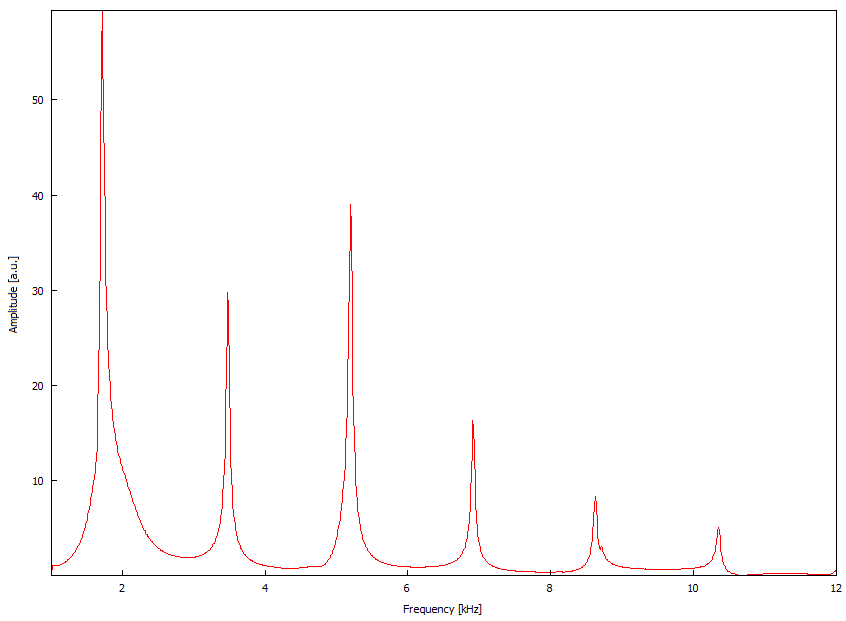
\includegraphics[width=\linewidth]{figure/2_Zylinder.png}
        \caption{Spektrum von zwei Zylindern\\ mittels \texttt{SpectrumSLC}}
     \end{minipage}
\end{figure}
%\FloatBarrier
%\FloatBarrier
\begin{figure}
    \begin{minipage}[b]{.4\linewidth} % [b] => Ausrichtung an \caption
        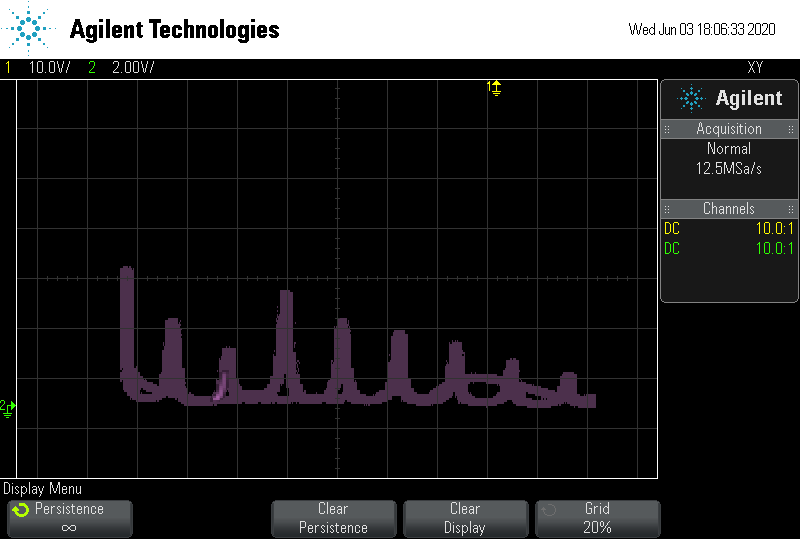
\includegraphics[width=\linewidth]{figure/3Zylinder.png}
        \vspace*{0.008cm}
        \caption{Spektrum von drei Zylindern\\ mittels Osziloskop}
     \end{minipage}
     \hspace{.1\linewidth}% Abstand zwischen Bilder
     \begin{minipage}[b]{.4\linewidth} % [b] => Ausrichtung an \caption
        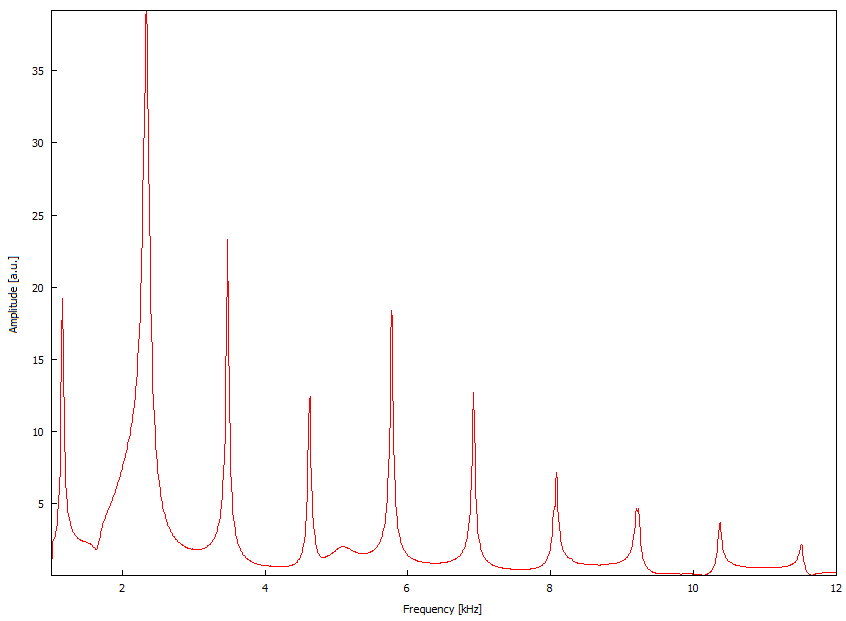
\includegraphics[width=\linewidth]{figure/3_Zylinder.png}
        \caption{Spektrum von drei Zylindern\\ mittels \texttt{SpectrumSLC}}
     \end{minipage}
\end{figure}
%\FloatBarrier
%\FloatBarrier
\begin{figure}
    \begin{minipage}[b]{.4\linewidth} % [b] => Ausrichtung an \caption
        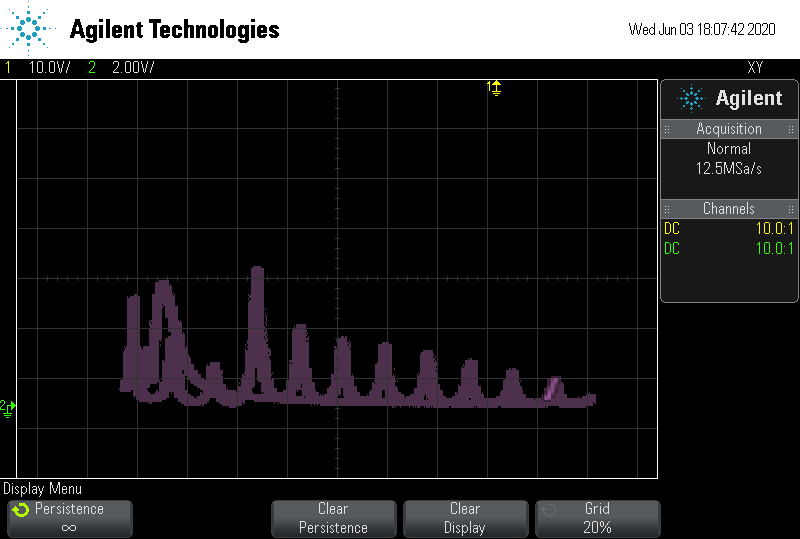
\includegraphics[width=\linewidth]{figure/4Zylinder.png}
        \vspace*{0.008cm}
        \caption{Spektrum von vier Zylindern\\ mittels Osziloskop}
     \end{minipage}
     \hspace{.1\linewidth}% Abstand zwischen Bilder
     \begin{minipage}[b]{.4\linewidth} % [b] => Ausrichtung an \caption
        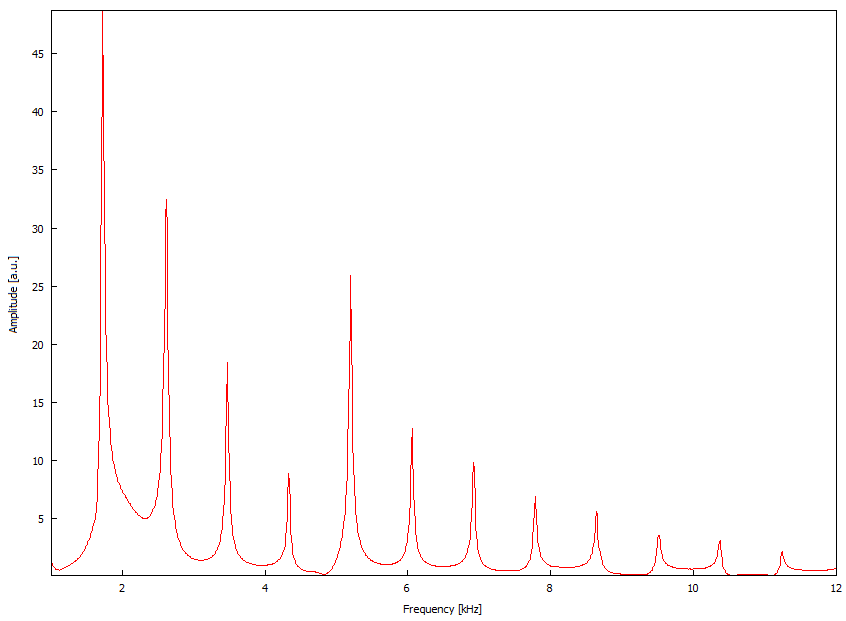
\includegraphics[width=\linewidth]{figure/4_Zylinder.png}
        \caption{Spektrum von vier Zylindern\\ mittels \texttt{SpectrumSLC}}
     \end{minipage}
\end{figure}
%\FloatBarrier
%\FloatBarrier
\begin{figure}
    \begin{minipage}[b]{.4\linewidth} % [b] => Ausrichtung an \caption
        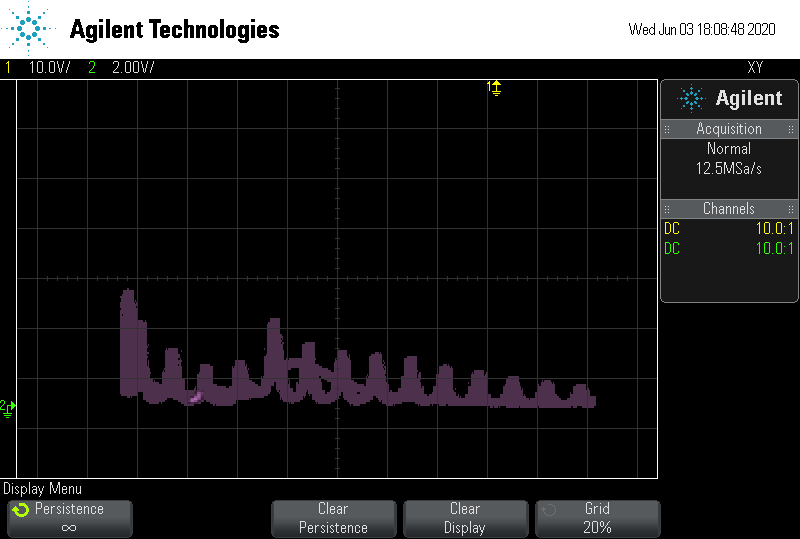
\includegraphics[width=\linewidth]{figure/5Zylinder.png}
        \vspace*{0.008cm}
        \caption{Spektrum von fünf Zylindern\\ mittels Osziloskop}
     \end{minipage}
     \hspace{.1\linewidth}% Abstand zwischen Bilder
     \begin{minipage}[b]{.4\linewidth} % [b] => Ausrichtung an \caption
        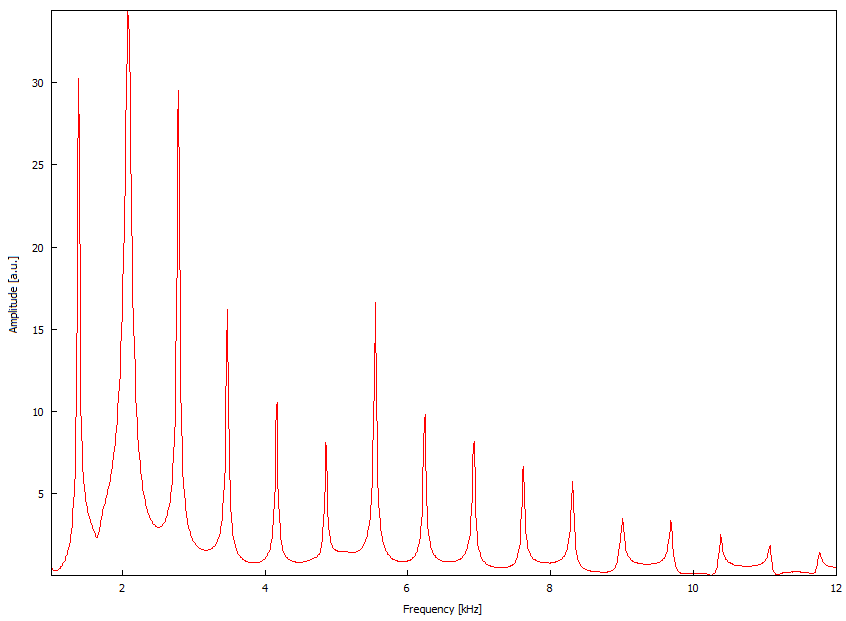
\includegraphics[width=\linewidth]{figure/5_Zylinder.png}
        \caption{Spektrum von fünf Zylindern\\ mittels \texttt{SpectrumSLC}}
     \end{minipage}
\end{figure}
%\FloatBarrier
%\FloatBarrier
\begin{figure}
    \begin{minipage}[b]{.4\linewidth} % [b] => Ausrichtung an \caption
        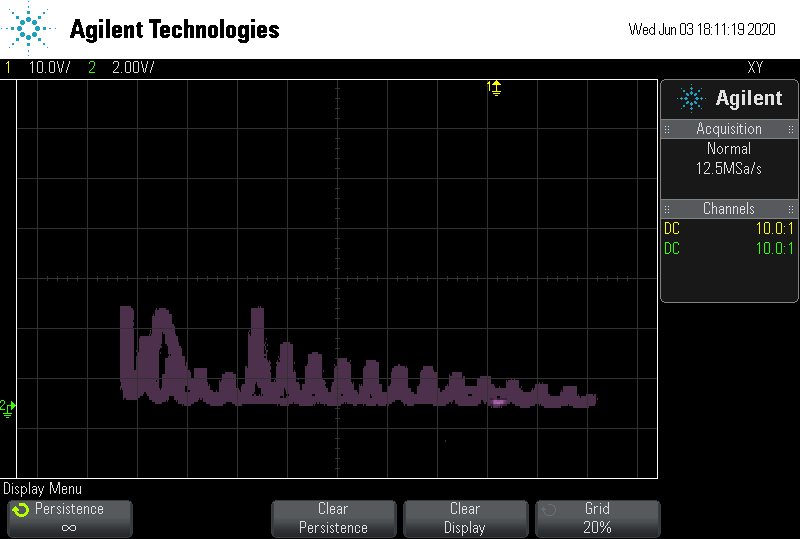
\includegraphics[width=\linewidth]{figure/6Zylinder.png}
        \vspace*{0.008cm}
        \caption{Spektrum von sechs Zylindern\\ mittels Osziloskop}
     \end{minipage}
     \hspace{.1\linewidth}% Abstand zwischen Bilder
     \begin{minipage}[b]{.4\linewidth} % [b] => Ausrichtung an \caption
        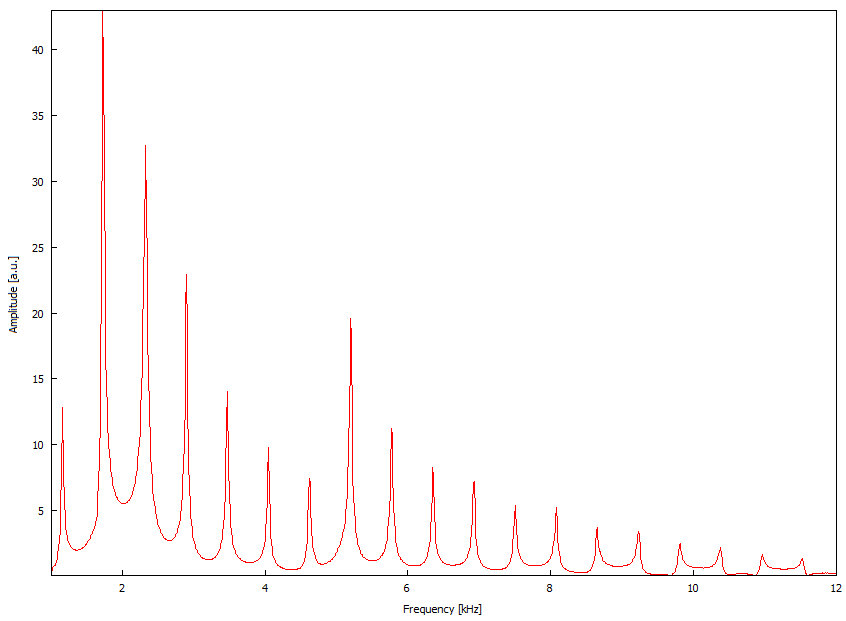
\includegraphics[width=\linewidth]{figure/6_Zylinder.png}
        \caption{Spektrum von sechs Zylindern\\ mittels \texttt{SpectrumSLC}}
     \end{minipage}
\end{figure}
\FloatBarrier

Wie an den Bildern erkannt werden kann, ist das Programm \texttt{SpectrumSLC} präzieser. Dazu kommt noch, dass das Programm die 
Daten abspeichert. Das kann die Auswertung der folgenden Messreihen vereinfachen.

\subsection{Das Wasserstoffmodel}
Für den ersten Versuch dieser Messreihe, sollen die Frequenzen von \SI{100}{\hertz} bis \SI{10}{\kilo\hertz} vermessen werden.
Die Resonanzfrequenzen sind in Tabelle \ref{tab:Resonanzfrequenzen} aufgelistet.
\FloatBarrier
\begin{table}
    \centering
    \caption{Messwertte für die Bestimmung der Ordnung der Resonanzfrequenz}
    \label{tab:Resonanzfrequenzen}
    \begin{tabular}{c c c c}
        \toprule
        Ordnung&Resonanzfrequenz /\SI{}{\kilo\hertz} &Amplitude /\SI{}{\milli\volt}& Phasenverschiebung /\SI{}{\degree}\\
        \midrule
        $\num{1}$&$\num{0.4376}$&$\num{160}$&$\num{0}-  \num{30}$\\
        $\num{2}$&$\num{2.3164}$&$\num{150}$&$\num{-20}-\num{4}$\\
        $\num{3}$&$\num{3.7095}$&$\num{150}$&$\num{-20}-\num{0}$\\
        $\num{4}$&$\num{5.0074}$&$\num{160}$&$\num{-20}-\num{0}$\\
        $\num{5}$&$\num{6.2361}$&$\num{160}$&$\num{-20}-\num{0}$\\
        $\num{6}$&$\num{6.5908}$&$\num{160}$&$\num{-20}-\num{4}$\\
        $\num{7}$&$\num{7.4648}$&$\num{160}$&$\num{-15}-\num{7}$\\
        $\num{8}$&$\num{8.0705}$&$\num{165}$&$\num{-20}-\num{0}$\\
        $\num{9}$&$\num{8.6602}$&$\num{170}$&$\num{-30}-(\num{-5})$\\
        $\num{10}$&$\num{9.5068}$&$\num{170}$&$\num{-30}-(\num{-5})$\\
        $\num{11}$&$\num{9.8462}$&$\num{175}$&$\num{-15}-\num{3}$\\
        \bottomrule
    \end{tabular}
\end{table}
\FloatBarrier
Die Resonanzen können auch mittels des Frequnezspektrometers dargestellt werden.
\FloatBarrier
\begin{figure}
    \caption{Frequnezspektrum des Kugelresonators}
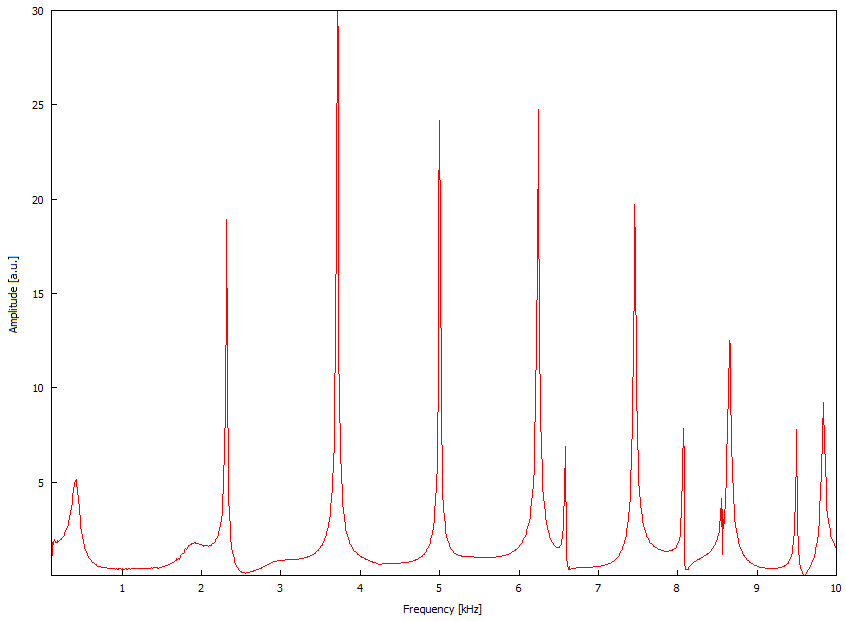
\includegraphics[width = \textwidth]{figure/Kugelresonanzspektrum.png}
\end{figure}

\subsubsection{Vermessung der Kugelflächenfunktion}
In dieser Messreihe werden für drei verschiedene Resonazen die Druckamplitude in Abhängigkeit des Drehwinkels $\alpha$ vermessen.
Es werden die Resonanzen der Ordnung 2,4 und 6 aus Tabelle \ref{tab:Resonanzfrequenzen} verwendet.
\FloatBarrier
\begin{table}
    \centering
    \caption{Messwertte für die Bestimmung der Ordnung der Kugelflächenfunktion}
    \label{tab:Amplituden_Kugelflächenfunktion}
    \begin{tabular}{c c c c c}
        \toprule
        Winkel $\alpha$ /\SI{}{\degree}&Winkel $\theta$ /\SI{}{\degree}&Amplitude 2 /\SI{}{\milli\volt}&Amplitude 4 /\SI{}{\milli\volt}& Amplitude 6 /\SI{}{\milli\volt}\\
        \midrule
        $\num{0}$  &$\num{90.0}$  &$\num{160}$&$\num{0.12}$&$\num{1.37}$\\
        $\num{10}$ &$\num{90.4}$ &$\num{160}$&$\num{0.68}$&$\num{1.45}$\\
        $\num{20}$ &$\num{91.7}$ &$\num{160}$&$\num{1.1}$&$\num{1.29}$\\
        $\num{30}$ &$\num{93.8}$ &$\num{160}$&$\num{1.4}$&$\num{1.05}$\\
        $\num{40}$ &$\num{96.7}$ &$\num{160}$&$\num{1.6}$&$\num{1.37}$\\
        $\num{50}$ &$\num{100.3}$ &$\num{160}$&$\num{2.0}$&$\num{1.21}$\\
        $\num{60}$ &$\num{104.5}$ &$\num{160}$&$\num{2.37}$&$\num{0.88}$\\
        $\num{70}$ &$\num{109.2}$ &$\num{160}$&$\num{2.61}$&$\num{0.8}$\\
        $\num{80}$ &$\num{114.4}$ &$\num{160}$&$\num{2.77}$&$\num{0.72}$\\
        $\num{90}$ &$\num{120.0}$ &$\num{160}$&$\num{2.7}$&$\num{0.84}$\\
        $\num{100}$&$\num{125.9}$&$\num{160}$&$\num{2.21}$&$\num{1.13}$\\
        $\num{110}$&$\num{132.1}$&$\num{160}$&$\num{1.45}$&$\num{1.37}$\\
        $\num{120}$&$\num{138.6}$&$\num{160}$&$\num{0.4}$&$\num{1.69}$\\
        $\num{130}$&$\num{145.2}$&$\num{160}$&$\num{1.29}$&$\num{2.01}$\\
        $\num{140}$&$\num{152.0}$&$\num{160}$&$\num{2.69}$&$\num{2.29}$\\
        $\num{150}$&$\num{158.9}$&$\num{160}$&$\num{4.34}$&$\num{2.61}$\\
        $\num{160}$&$\num{165.9}$&$\num{160}$&$\num{5.3}$&$\num{2.85}$\\
        $\num{170}$&$\num{172.9}$&$\num{160}$&$\num{6.03}$&$\num{3.34}$\\
        $\num{180}$&$\num{180.0}$&$\num{160}$&$\num{6.43}$&$\num{3.26}$\\
        \bottomrule
    \end{tabular}
\end{table}
\FloatBarrier
In der Tabelle \ref{tab:Amplituden_Kugelflächenfunktion} wird der Winkel $\theta$ mit der Funktion \eqref{eq:Theta_alpha} aus $\alpha$ bestimmt.
\begin{equation}
    \label{eq:Theta_alpha}
    \theta(\alpha) = \arccos\left( \frac{1}{2} \cos\left( \alpha \right) -\frac{1}{2} \right)
\end{equation}
Wie aus Tabelle \ref{tab:Amplituden_Kugelflächenfunktion} abzulesen ist, ist die Druckamplitude der zweiten Resonanz 
unabhängig von dem Winkel, daher müssen die Quantenzahlen $n=m=0$ sein.\\
Die Druckamplitude wird gegen $\theta$ in einem Polarplot aufgetragen. Dazu werden verschiedene Kugelflächenfunktionen 
geplottet, um diese miteinander vergleichen zu können. Da ohne Zwischenring keine Aufspaltung in $m$ zu sehen ist, wird $m=0$ gesetzt,
um die Kugelflächenfunktion nur in Abhängigkeit von $\theta$ zu plotten.
\FloatBarrier
\begin{figure}
    \hspace*{2cm}
    \begin{minipage}[b]{.4\linewidth} % [b] => Ausrichtung an \caption
        \hspace*{-2cm}
        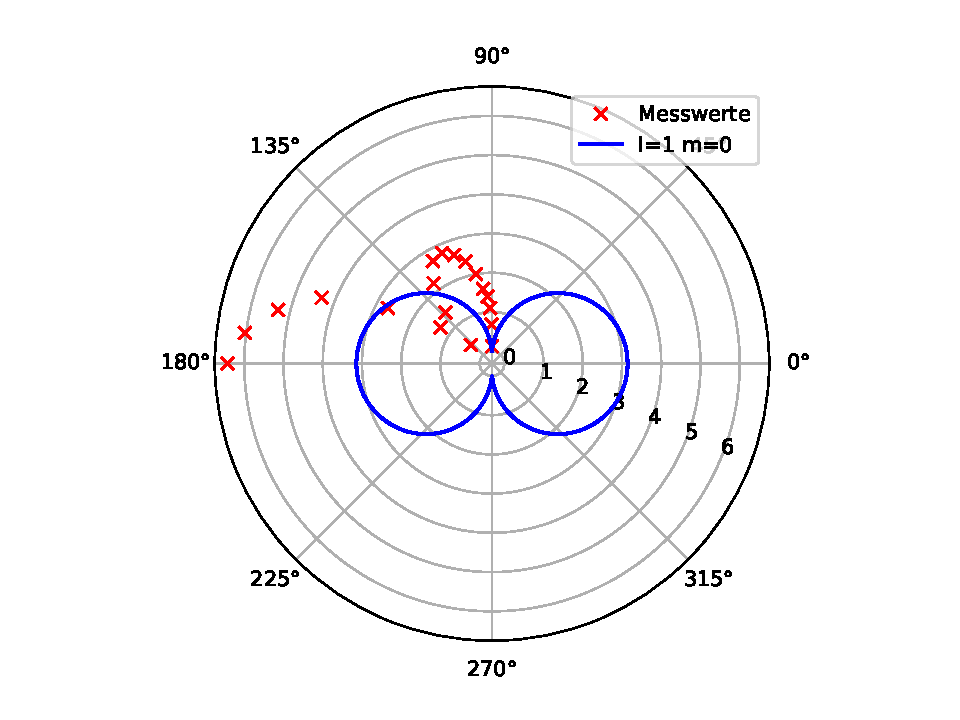
\includegraphics[width=\linewidth]{figure/Resonanz_Drewinkel_Amplitude_4_n1.pdf}
        \caption{Winkelabhängigkeit der\\ Druckamplitude bei einer \\ Resonanzfrequenz von \SI{5.0074}{\kilo\hertz} und \\ Kugelflächenfunktion der ersten Ordnung.}
        \label{fig:Resonanz_Drewinkel_Amplitude_4_n1}
     \end{minipage}
     \hspace{.1\linewidth}% Abstand zwischen Bilder
     \begin{minipage}[b]{.4\linewidth} % [b] => Ausrichtung an \caption
        \hspace*{-2cm}
        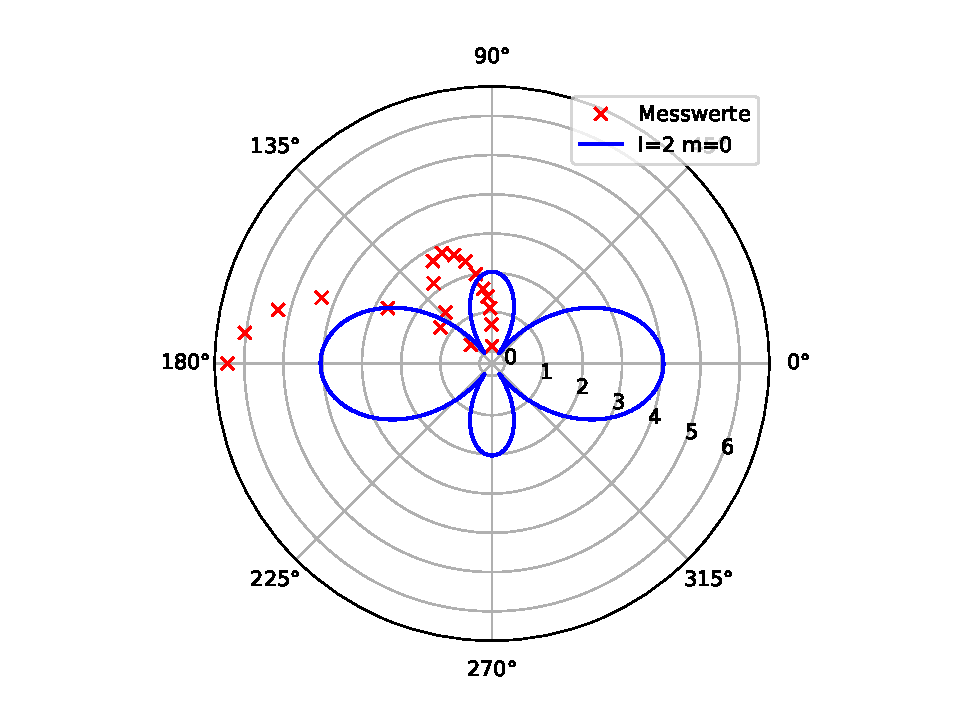
\includegraphics[width=\linewidth]{figure/Resonanz_Drewinkel_Amplitude_4_n2.pdf}
        \caption{Winkelabhängigkeit der\\ Druckamplitude bei einer \\ Resonanzfrequenz von \SI{5.0074}{\kilo\hertz} und \\ Kugelflächenfunktion der zweiten Ordnung.}
     \end{minipage}
\end{figure}
\begin{figure}
    \hspace*{2cm}
    \begin{minipage}[b]{.4\linewidth} % [b] => Ausrichtung an \caption
        \hspace*{-2cm}
        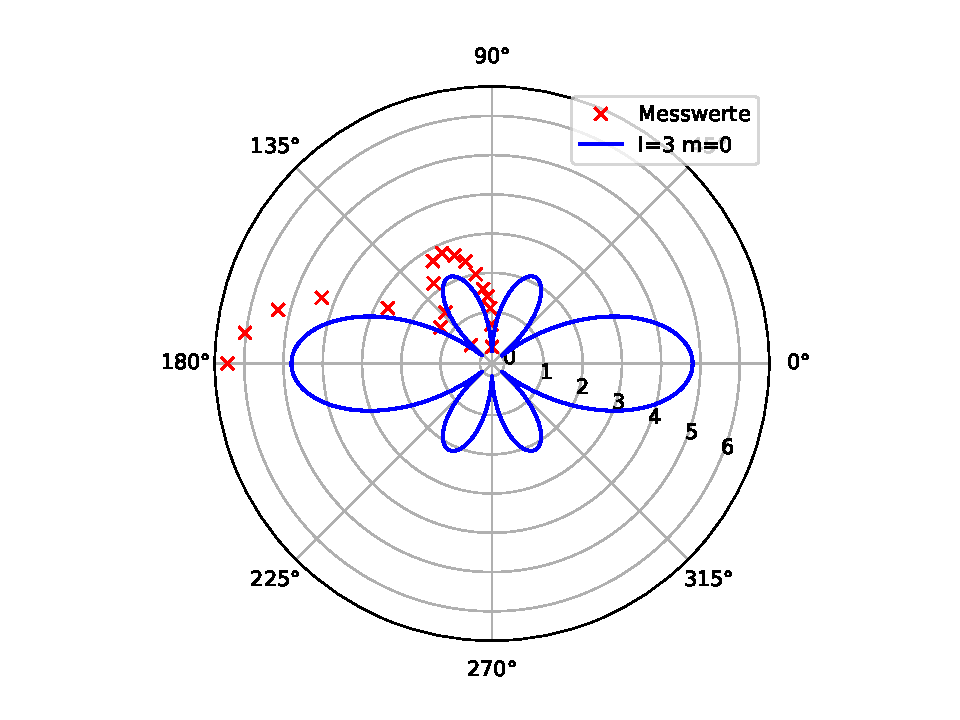
\includegraphics[width=\linewidth]{figure/Resonanz_Drewinkel_Amplitude_4_n3.pdf}
        \caption{Winkelabhängigkeit der\\ Druckamplitude bei einer \\ Resonanzfrequenz von \SI{5.0074}{\kilo\hertz} und \\ Kugelflächenfunktion der dritten Ordnung.}
     \end{minipage}
     \hspace{.1\linewidth}% Abstand zwischen Bilder
     \begin{minipage}[b]{.4\linewidth} % [b] => Ausrichtung an \caption
        \hspace*{-2cm}
        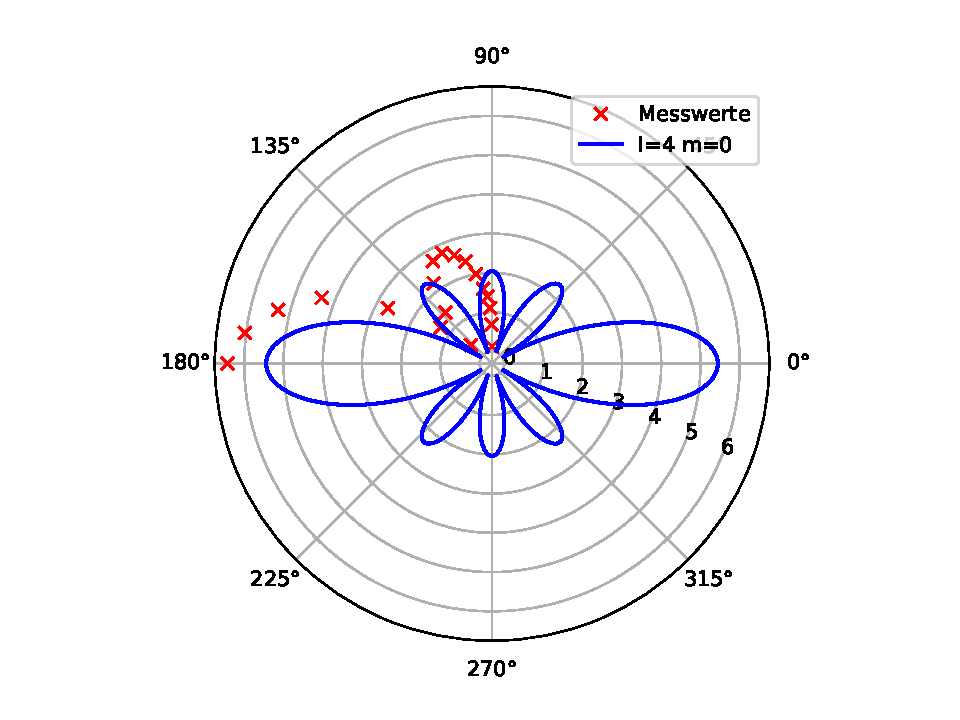
\includegraphics[width=\linewidth]{figure/Resonanz_Drewinkel_Amplitude_4_n4.pdf}
        \caption{Winkelabhängigkeit der\\ Druckamplitude bei einer \\ Resonanzfrequenz von \SI{5.0074}{\kilo\hertz} und \\ Kugelflächenfunktion der vierten Ordnung.}
        \label{fig:fig:Resonanz_Drewinkel_Amplitude_4_n4}
     \end{minipage}
\end{figure}


\begin{figure}
    \hspace*{2cm}
    \begin{minipage}[b]{.4\linewidth} % [b] => Ausrichtung an \caption
        \hspace*{-2cm}
        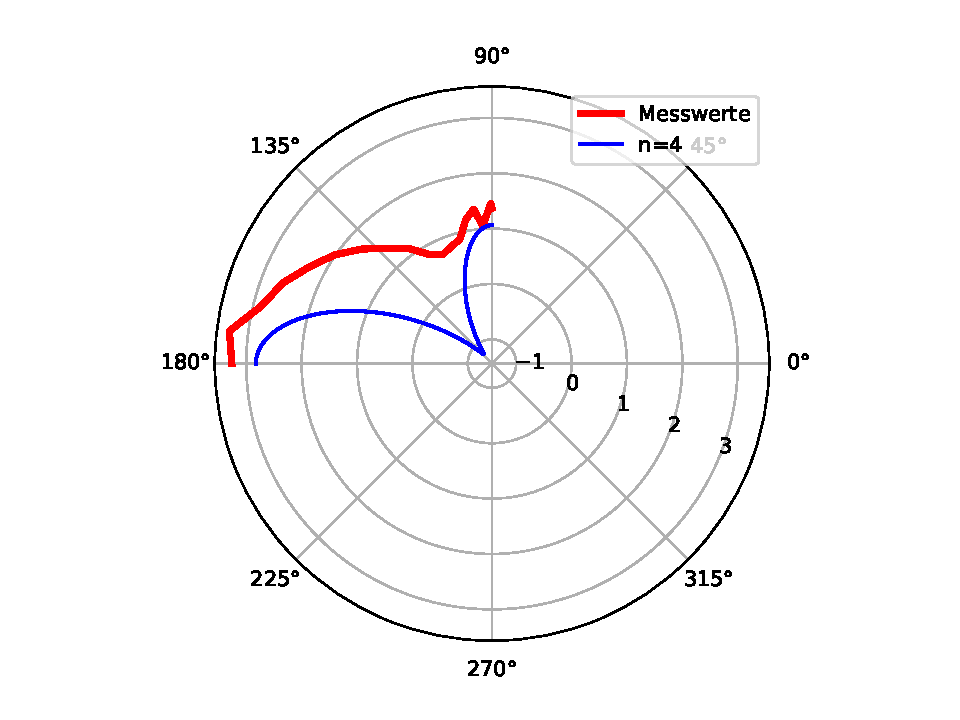
\includegraphics[width=\linewidth]{figure/Resonanz_Drewinkel_Amplitude_6_n4.pdf}
        \caption{Winkelabhängigkeit der\\ Druckamplitude bei einer \\ Resonanzfrequenz von \SI{6.5908}{\kilo\hertz} und \\ Kugelflächenfunktion der vierten Ordnung.}
        \label{fig:fig:Resonanz_Drewinkel_Amplitude_6_n4}
     \end{minipage}
     \hspace{.1\linewidth}% Abstand zwischen Bilder
     \begin{minipage}[b]{.4\linewidth} % [b] => Ausrichtung an \caption
        \hspace*{-2cm}
        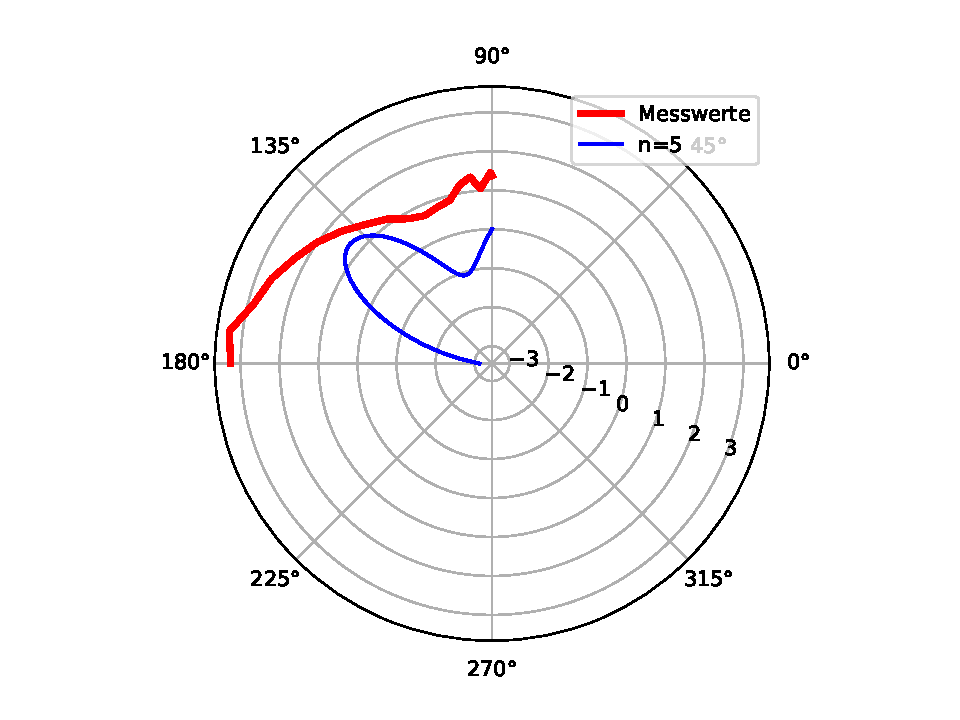
\includegraphics[width=\linewidth]{figure/Resonanz_Drewinkel_Amplitude_6_n5.pdf}
        \caption{Winkelabhängigkeit der\\ Druckamplitude bei einer \\ Resonanzfrequenz von \SI{6.5908}{\kilo\hertz} und \\ Kugelflächenfunktion der fünften Ordnung.}
     \end{minipage}
\end{figure}
\begin{figure}
    \hspace*{2cm}
    \begin{minipage}[b]{.4\linewidth} % [b] => Ausrichtung an \caption
        \hspace*{-2cm}
        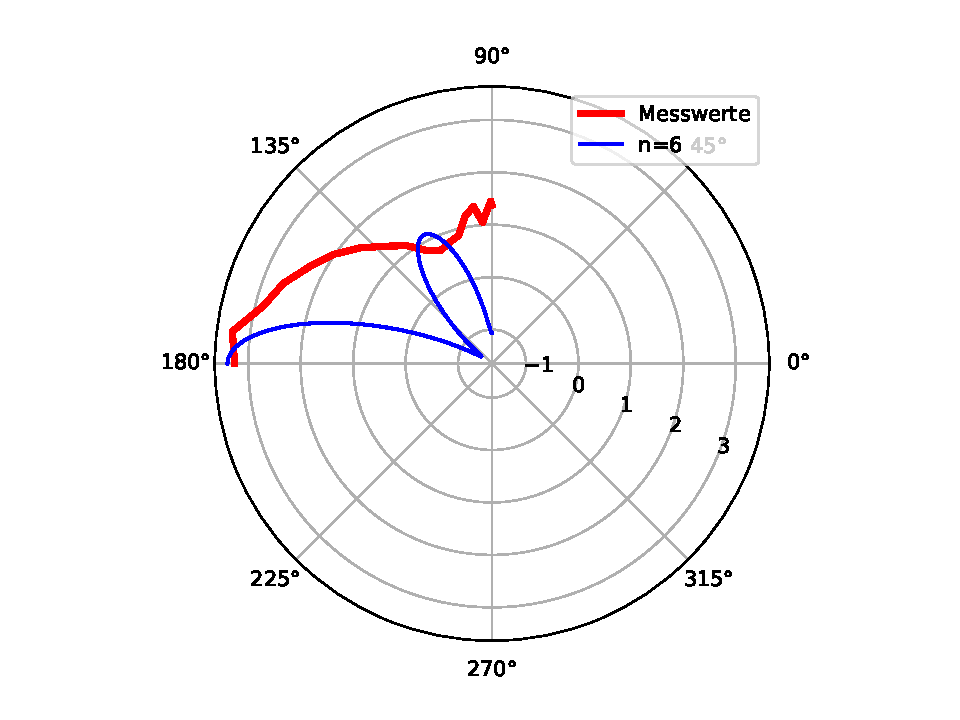
\includegraphics[width=\linewidth]{figure/Resonanz_Drewinkel_Amplitude_6_n6.pdf}
        \caption{Winkelabhängigkeit der\\ Druckamplitude bei einer \\ Resonanzfrequenz von \SI{6.5908}{\kilo\hertz} und \\ Kugelflächenfunktion der sechsten Ordnung.}
     \end{minipage}
     \hspace{.1\linewidth}% Abstand zwischen Bilder
     \begin{minipage}[b]{.4\linewidth} % [b] => Ausrichtung an \caption
        \hspace*{-2cm}
        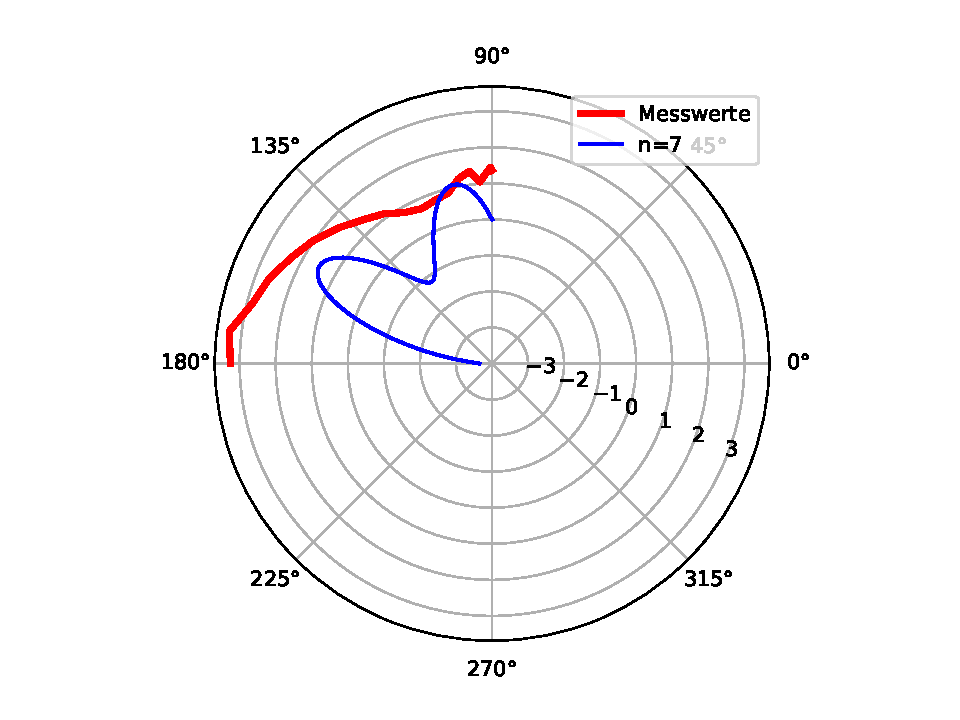
\includegraphics[width=\linewidth]{figure/Resonanz_Drewinkel_Amplitude_6_n7.pdf}
        \caption{Winkelabhängigkeit der\\ Druckamplitude bei einer \\ Resonanzfrequenz von \SI{6.5908}{\kilo\hertz} und \\ Kugelflächenfunktion der siebten Ordnung.}
        \label{fig:Resonanz_Drewinkel_Amplitude_6_n7}
     \end{minipage}
\end{figure}
\FloatBarrier
Bei Betrachtung von Abbildung \ref{fig:Resonanz_Drewinkel_Amplitude_4_n1} bis (??)[muss manuel eingefühgt werden] kann gesagt werden, 
dass die gemessene Verteilung der Kugelflächenfunktion mit $n=4$ ähnelt. \\
Da die Verteilung bei Abbildung (??)[auch hier manuel] bis \ref{fig:Resonanz_Drewinkel_Amplitude_6_n7}  keiner der Kugelflächenfunktion ähnelt, aber
$n>4$ sein muss, kann die Kugelflächenfunktion nicht bestimmt werden.
\subsubsection{Peakaufspaltung}
Bei dieser Messreihe wird die Peakaufspaltung der Resonanzfrequenz von \SI{2.3}{\kilo\hertz} vermessen, indem verschieden dicke 
Zwischenringe zwischen den Halbkugeln des Kugelresonators eigefühgt werden.
Die dafür benötigten Messdaten sind in Tabelle  aufgelistet.
\FloatBarrier
\begin{table}
    \centering
    \caption{Messwerte für die Bestimmung des Zusammenhangs zwischen der Dicke des Zwischerings und der Aufspaltung der Resonanzfrequenz}
    %\label{tab:Peakaufspaltung}
    \begin{tabular}{c c c c}
        \toprule
        Dicke / \SI{}{\milli\meter}& erster Resonanz / \SI{}{\kilo\hertz}& zweite Resonanz / \SI{}{\kilo\hertz}& Differenz / \SI{}{\kilo\hertz}\\
        \midrule
        $\num{3}$ &$\num{2239}$&$\num{2302}$&$\num{63}$\\
        $\num{9}$ &$\num{2173}$&$\num{2286}$&$\num{113}$\\
        $\num{12}$&$\num{2103}$&$\num{2277}$&$\num{174}$\\
        \bottomrule
    \end{tabular}
\end{table}
\FloatBarrier
Aufgrund der wenigen Kombinationsmöglichkeiten der beiden Zwischenring, können für diesen Versuch nur drei Messwerte aufgenommen werden.
Da aus drei Punkten nicht auf komplexe Funktionen geschlossen werden kann wird der Zusammenhang linear angenommen.
Dafür wird die Funktion \eqref{eq:linear} durch die Daten gefittet.
\begin{equation}
    f\left(x\right) = ax +b
    \label{eq:linear}
\end{equation}
\FloatBarrier
\begin{figure}
    \centering
    \caption{Messdaten und Fit für den Zusammenhang zwischen Zwischenringdicke und Peakaufspaltung}
    \label{fig:Peakaufspaltung}
    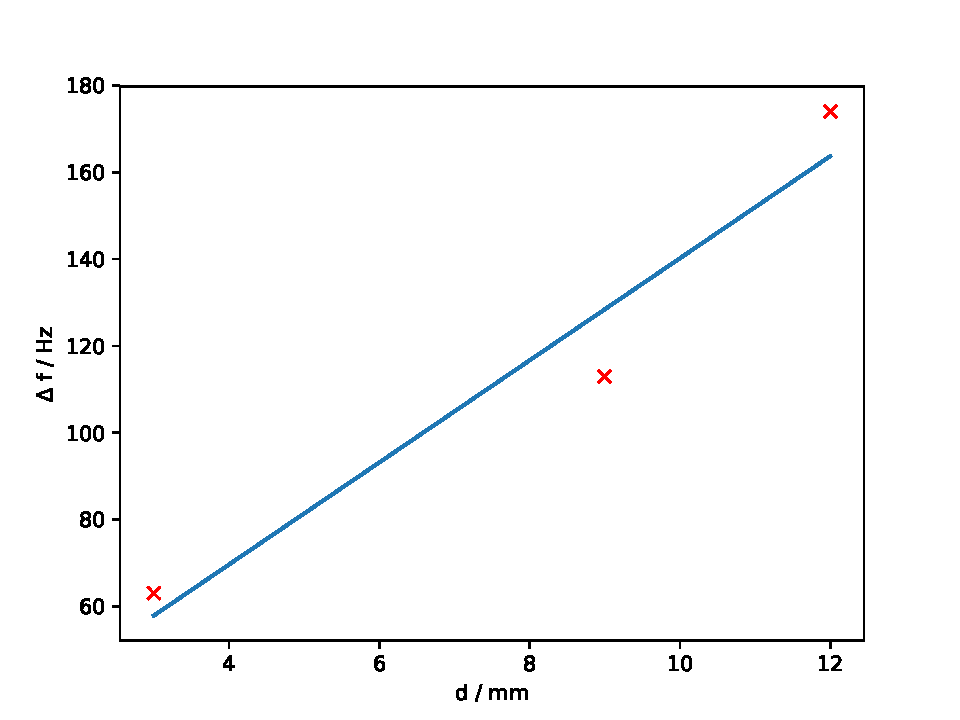
\includegraphics[width=0.7\textwidth]{figure/Peak_Aufspaltung.pdf}
\end{figure}
\FloatBarrier
In der Abbildung \ref{fig:Peakaufspaltung} sind die Parameter auf 
\begin{align*}
    a&= \num{12(3)}\\
    b&= \num{23(26)}
\end{align*}
bestimmt worden
\subsubsection{Bestimmung des Quantenzustandes}
Um die Quantenzahlen des Zustandes zu bestimmen, wird ein Zwischenring der Dicke von $d=\SI{9}{\milli\meter}$ eigefühgt.
Da der Zwischenring die Symmetrie der Kugel bricht gibt es jetzt eine Vorzugsrichtung. Dadurch ist der $\alpha$-Winkel der $\Phi$ Winkel 
der Kugelflächenfunktion und die Ausrichtung des Mikrofons ist der $\theta$-Winkel.
Bei einer Frequenzen von \SI{2.3}{\kilo\hertz} wird die winkelabhängige Druckamplitude vermessen. Die Messdaten sind in Tabelle
\ref{tab:Messdaten_9mmZwischenring} aufgelistet.
\FloatBarrier
\begin{table}
    \centering
    \caption{Messwerte für die Bestimmung des Quantenzustandes bei einer Resonanzfrequenz von \SI{2.3}{\kilo\hertz} und einem Zwischenring der Dick $d=\SI{9}{\milli\meter}$.}
    \label{tab:Messdaten_9mmZwischenring}
    \begin{tabular}{c c c c c}
        \toprule
        Winkel $\phi$ /\SI{}{\degree}&Amplitude  /\SI{}{\milli\volt}\\
        \midrule
        $\num{0}$  &$\num{640}$ \\
        $\num{10}$ &$\num{640}$ \\
        $\num{20}$ &$\num{600}$ \\
        $\num{30}$ &$\num{560}$ \\
        $\num{40}$ &$\num{480}$ \\
        $\num{50}$ &$\num{400}$\\
        $\num{60}$ &$\num{320}$\\
        $\num{70}$ &$\num{220}$\\
        $\num{80}$ &$\num{125}$\\
        $\num{90}$ &$\num{120}$\\
        $\num{100}$&$\num{233}$\\
        $\num{110}$&$\num{350}$\\
        $\num{120}$&$\num{440}$\\
        $\num{130}$&$\num{520}$\\
        $\num{140}$&$\num{590}$\\
        $\num{150}$&$\num{675}$\\
        $\num{160}$&$\num{700}$\\
        $\num{170}$&$\num{760}$\\
        $\num{180}$&$\num{780}$\\
        \bottomrule
    \end{tabular}
\end{table}
\FloatBarrier
\begin{figure}
    \hspace*{2cm}
    \begin{minipage}[b]{.4\linewidth} % [b] => Ausrichtung an \caption
        \hspace*{-2cm}
        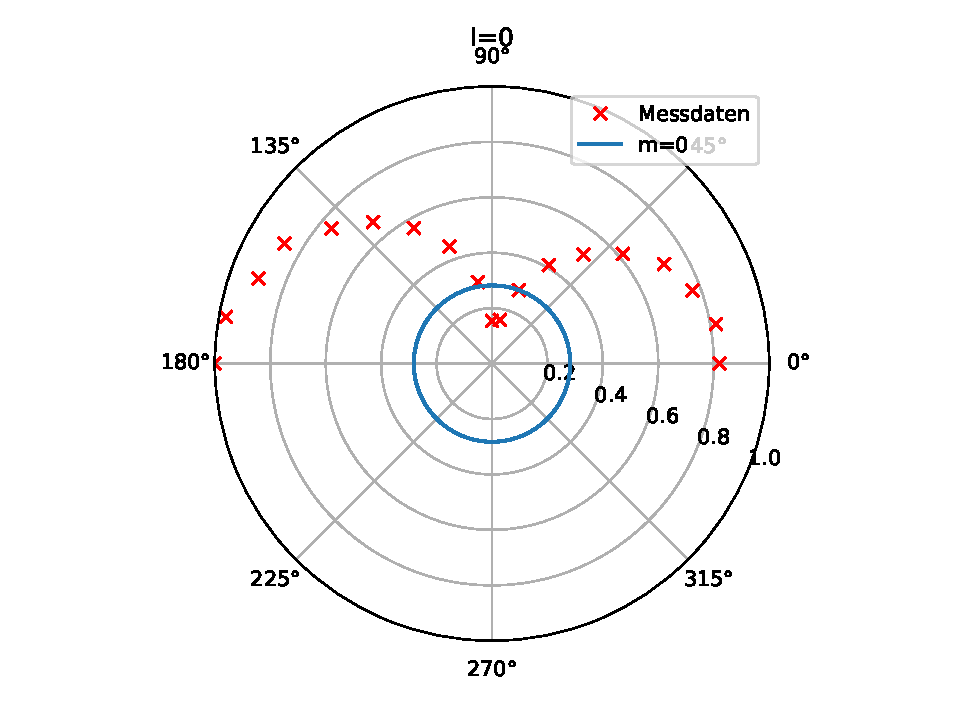
\includegraphics[width=\linewidth]{figure/9mmZwischenring_n0.pdf}
        \caption{Winkelabhängigkeit der\\ Druckamplitude bei einer \\ Resonanzfrequenz von \SI{2.3}{\kilo\hertz} und \\ Kugelflächenfunktionen der nullten Ordnung.}
     \end{minipage}
     \hspace{.1\linewidth}% Abstand zwischen Bilder
     \begin{minipage}[b]{.4\linewidth} % [b] => Ausrichtung an \caption
        \hspace*{-2cm}
        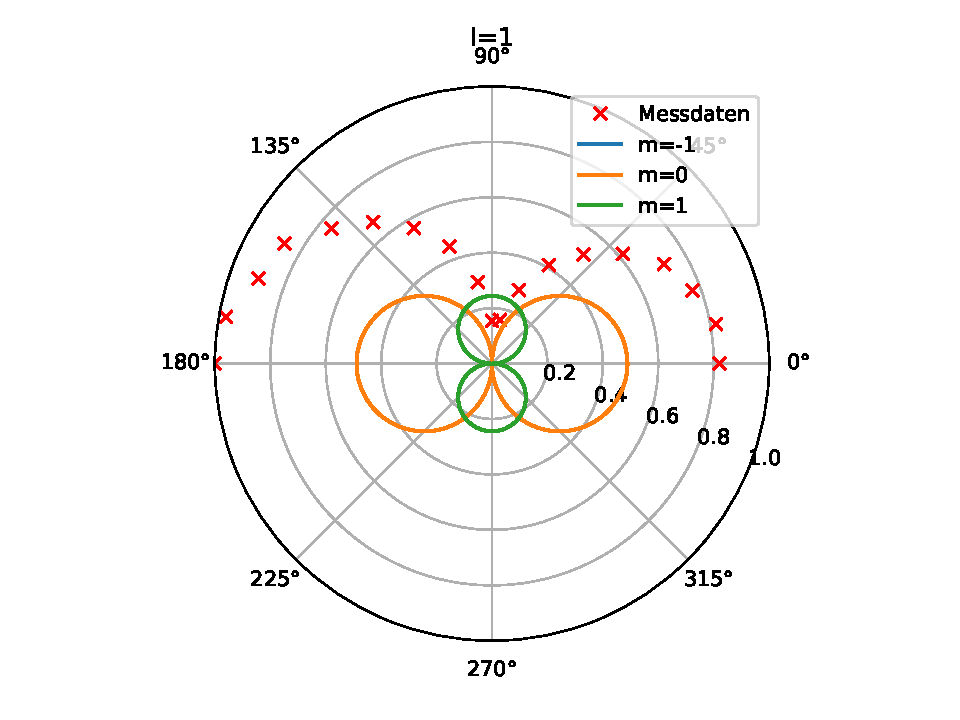
\includegraphics[width=\linewidth]{figure/9mmZwischenring_n1.pdf}
        \caption{Winkelabhängigkeit der\\ Druckamplitude bei einer \\ Resonanzfrequenz von \SI{2.3}{\kilo\hertz} und \\ Kugelflächenfunktionen der erste Ordnung.}
     \end{minipage}
\end{figure}
\begin{figure}
    \centering
    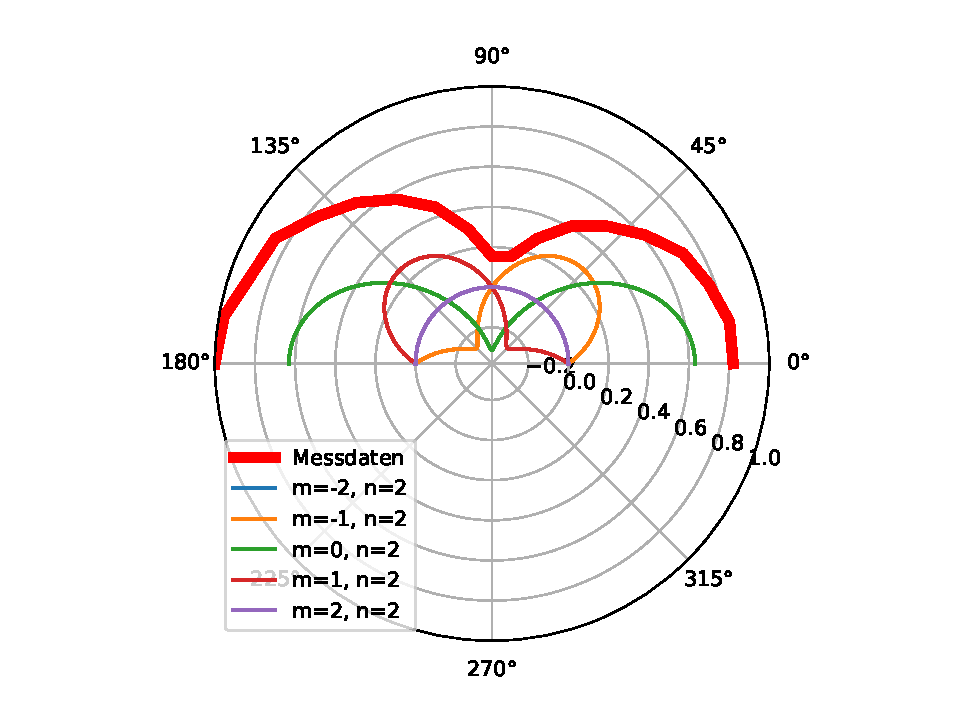
\includegraphics[width=0.5\textwidth]{figure/9mmZwischenring_n2.pdf}
    \caption{Winkelabhängigkeit der Druckamplitude bei einer Resonanzfrequenz von \SI{2.3}{\kilo\hertz} und Kugelflächenfunktionen der zweiten Ordnung.}
    \label{fig:9mmZwischenring_n2}
\end{figure}
\FloatBarrier
Wie an der Abbildung \ref{fig:9mmZwischenring_n2} zu sehen ist, ähnelt der Zustand am meisten der $n=2,m=0$ Kugelflächenfunktion.
\subsection{Das Wasserstoffmolekül}
Für die folgenden Versuchsteilen werden zwei Kugelresonatoren übereinander gesteckt und mit einem Loch in der Mitte in Verbindung gebracht.
\subsubsection{Resonanzfrequenz in Abhängigkeit des Blendendurchmessers}
Da nur zwei Blenden zu Verfügung standen, kann auch hier nur ein linearer Zusammenhang in erwägung gezogen werden.
Die beiden Spektren werden mit einer Blende mit einem Durchmesser von $d=\SI{10}{\milli\meter}$ und
$d=\SI{16}{\milli\meter}$ aufgenommen. Die Spektren sind in Abbildung \ref{fig:Spektren_WM_Blende} zu sehen.
\FloatBarrier
\begin{figure}
    \centering
    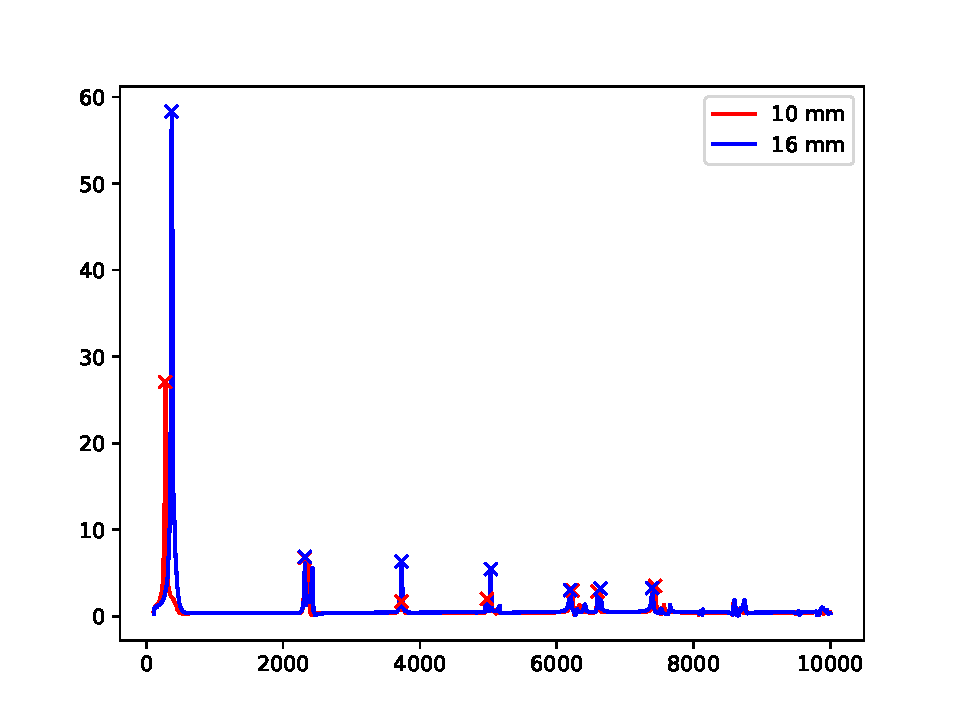
\includegraphics[width = 0.7\textwidth , keepaspectratio]{figure/WM_Blenden.pdf}
    \caption{Spektren für den Zusammenhang zwischen den Resonanzfrequenzen und dem Blendendurchmesser.}
    \label{fig:Spektren_WM_Blende}
\end{figure}
\FloatBarrier
Die Resonanzen sind in Tabelle \ref{tab:Resonanz_WM_Blenden} aufgelistet.
\FloatBarrier
\begin{table}
    \centering
    \caption{Resonanzen für den Zusammenhang zwischen Resonanzfrequenz und Blendendurchmesser.}
    \label{tab:Resonanz_WM_Blenden}
    \begin{tabular}{c c c}
        \toprule
        Durchmesser $d=\SI{10}{\milli\meter}$ &Durchmesser $d=\SI{16}{\milli\meter}$& \\
        Frequenz $f /\SI{}{\hertz}$& Frequenz $f /\SI{}{\hertz}$&Differenz $\Delta f /\SI{}{\hertz}$\\
        \midrule
        $\num{280}$ &$\num{370}$ &$\num{90}$\\
        $\num{2320}$&$\num{2320}$&$\num{0}$\\
        $\num{3730}$&$\num{3730}$&$\num{0}$\\
        $\num{4980}$&$\num{5040}$&$\num{60}$\\
        $\num{6230}$&$\num{6200}$&$\num{-30}$\\
        $\num{6600}$&$\num{6640}$&$\num{40}$\\
        $\num{7440}$&$\num{7400}$&$\num{-40}$\\
        \bottomrule
    \end{tabular}
\end{table}
\FloatBarrier
Wie an den den Differenzen aus Tabelle \ref{tab:Resonanz_WM_Blenden} zu erkennen ist, kann an diesen Daten kein 
Zusammenhang zwischen Blendendurchmesser und Resonanz gezogen werden.

\subsubsection{Quantenzustand des Wasserstoffmolekül}
Für die Bestimmung des Quantenzustandes des Wasserstoffmoleküls wird die Druckamplitude in Abhängigkeit des Drehwinkels 
vermessen. Hierbei ist die Frequenz auf \SI{2.3}{\kilo\hertz} eingestellt.
Die gemessenen Daten sind in Tabelle \ref{tab:WMQZ} aufgelistet.
\FloatBarrier
\begin{table}
    \centering
    \caption{Daten für die Bestimmung des Quantenzustandes des Wasserstoffmoleküls.}
    \label{tab:WMQZ}
    \begin{tabular}{c c}
        \toprule
        Drehwinkel $\alpha / \SI{}{\degree}$ & Druckamplitude / \SI{}{\volt}\\
        \midrule
        $\num{0}$  &$\num{1.05}$\\
        $\num{10}$ &$\num{1.05}$\\
        $\num{20}$ &$\num{0.96}$\\
        $\num{30}$ &$\num{0.96}$\\
        $\num{40}$ &$\num{0.96}$\\
        $\num{50}$ &$\num{0.88}$\\
        $\num{60}$ &$\num{0.88}$\\
        $\num{70}$ &$\num{0.88}$\\
        $\num{80}$ &$\num{0.84}$\\
        $\num{90}$ &$\num{0.84}$\\
        $\num{100}$&$\num{0.8}$\\
        $\num{110}$&$\num{0.8}$\\
        $\num{120}$&$\num{0.8}$\\
        $\num{130}$&$\num{0.72}$\\
        $\num{140}$&$\num{0.72}$\\
        $\num{150}$&$\num{0.72}$\\
        $\num{160}$&$\num{0.72}$\\
        $\num{170}$&$\num{0.72}$\\
        $\num{180}$&$\num{0.72}$\\
        \bottomrule
    \end{tabular}
\end{table}
\FloatBarrier
Die Daten werden in Abbildung \ref{fig:WMQZ} dargestellt.
\FloatBarrier
\begin{figure}
    \centering
    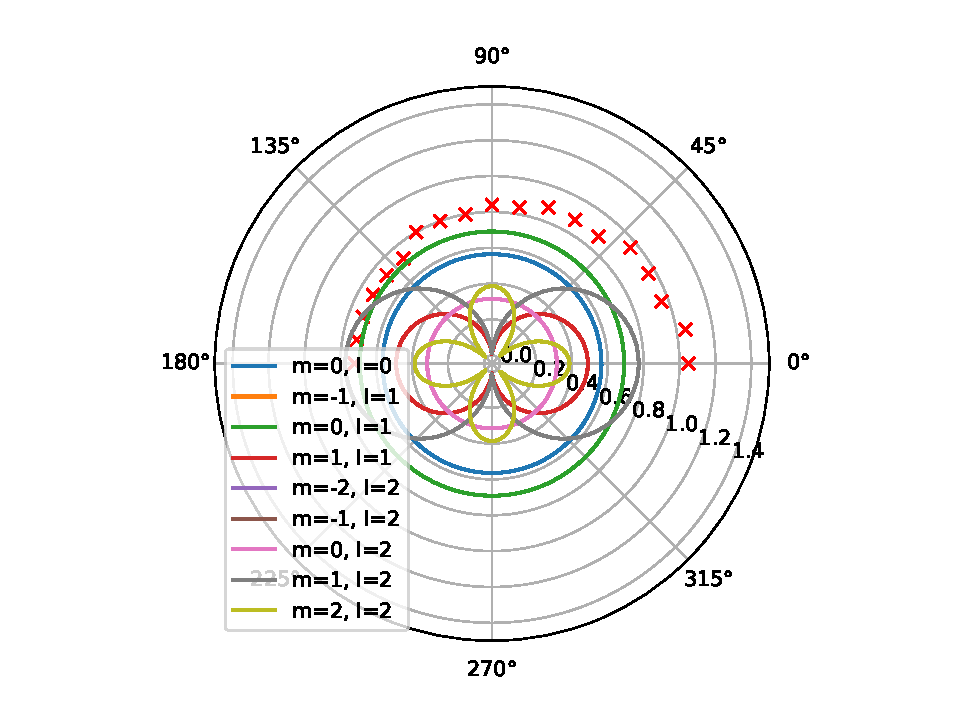
\includegraphics[width = 0.7\textwidth, keepaspectratio]{figure/WMQZ.pdf}
    \caption{Messdaten und verschiedene Kugelflächenfunktionen, für die Bestimmung des Quantenzustandes.}
    \label{fig:WMQZ}
\end{figure}
\FloatBarrier
Wie in der Abbildung \ref{fig:WMQZ} zu sehen ist, ähnelt der Vermessene Zustand der Kugelflächenfunktion mit 
$n=m=0$, $n=1 m=-1$ oder $n=2 m=2$. Da die zweite Resonanz verwendet wurde kann davon ausgegangen werden, das der 
$n=1 m=-1$ Zustand zutrifft. Das ist der $1\pi$ Zustand. Allerdings kann nicht gesagt werden ob dieser bindend oder antibindend 
ist.